\chapter{Appendix}
\label{ch:app:physics}

\section{Jet ID Efficiency}

The jet ID selection ensures a high purity of real jet events while keeping more than 99\% of the real jets.
The efficiency of the jet id is studied using a tag-and-probe approach. Well balanced jets in $\phi$ are selected
using a criteria of $\Delta \phi > 2.7$. While one jet needs to pass the tight jet id criteria, the balanced jet is probed
if if satisfies the criteria as well. The ratio of events where the probe jet passes the criteria versus the number of events
in which the probe doesn't pass the critera is used to estimate the efficiency. The efficiency is plotted as a function of the
dijet \ptavg as can be seen in Figure~\ref{fig:jetid_eff}. The efficiency is in all bins larger than 99\%.

\begin{figure}[htbp]
    \centering
    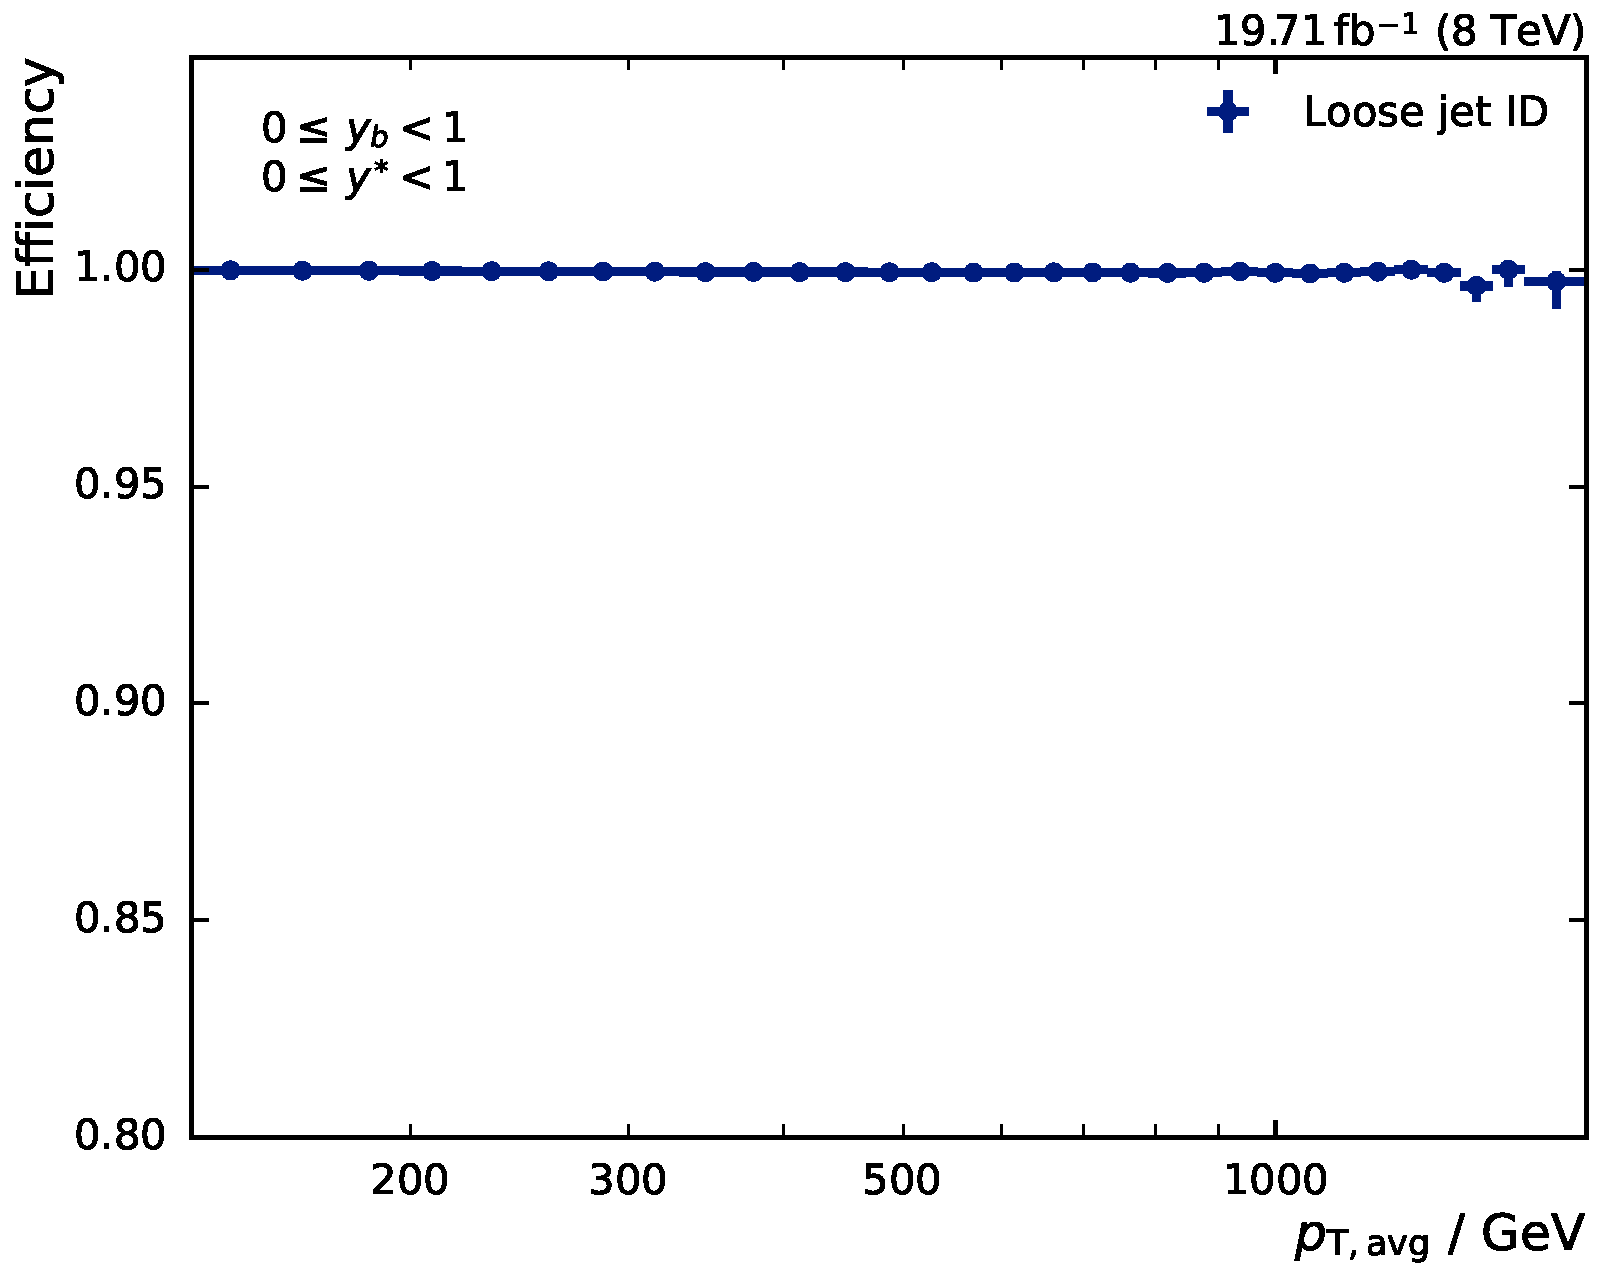
\includegraphics[width=0.45\textwidth]{figures/measurement/jetideff_yb0ys0.pdf}\hfill
    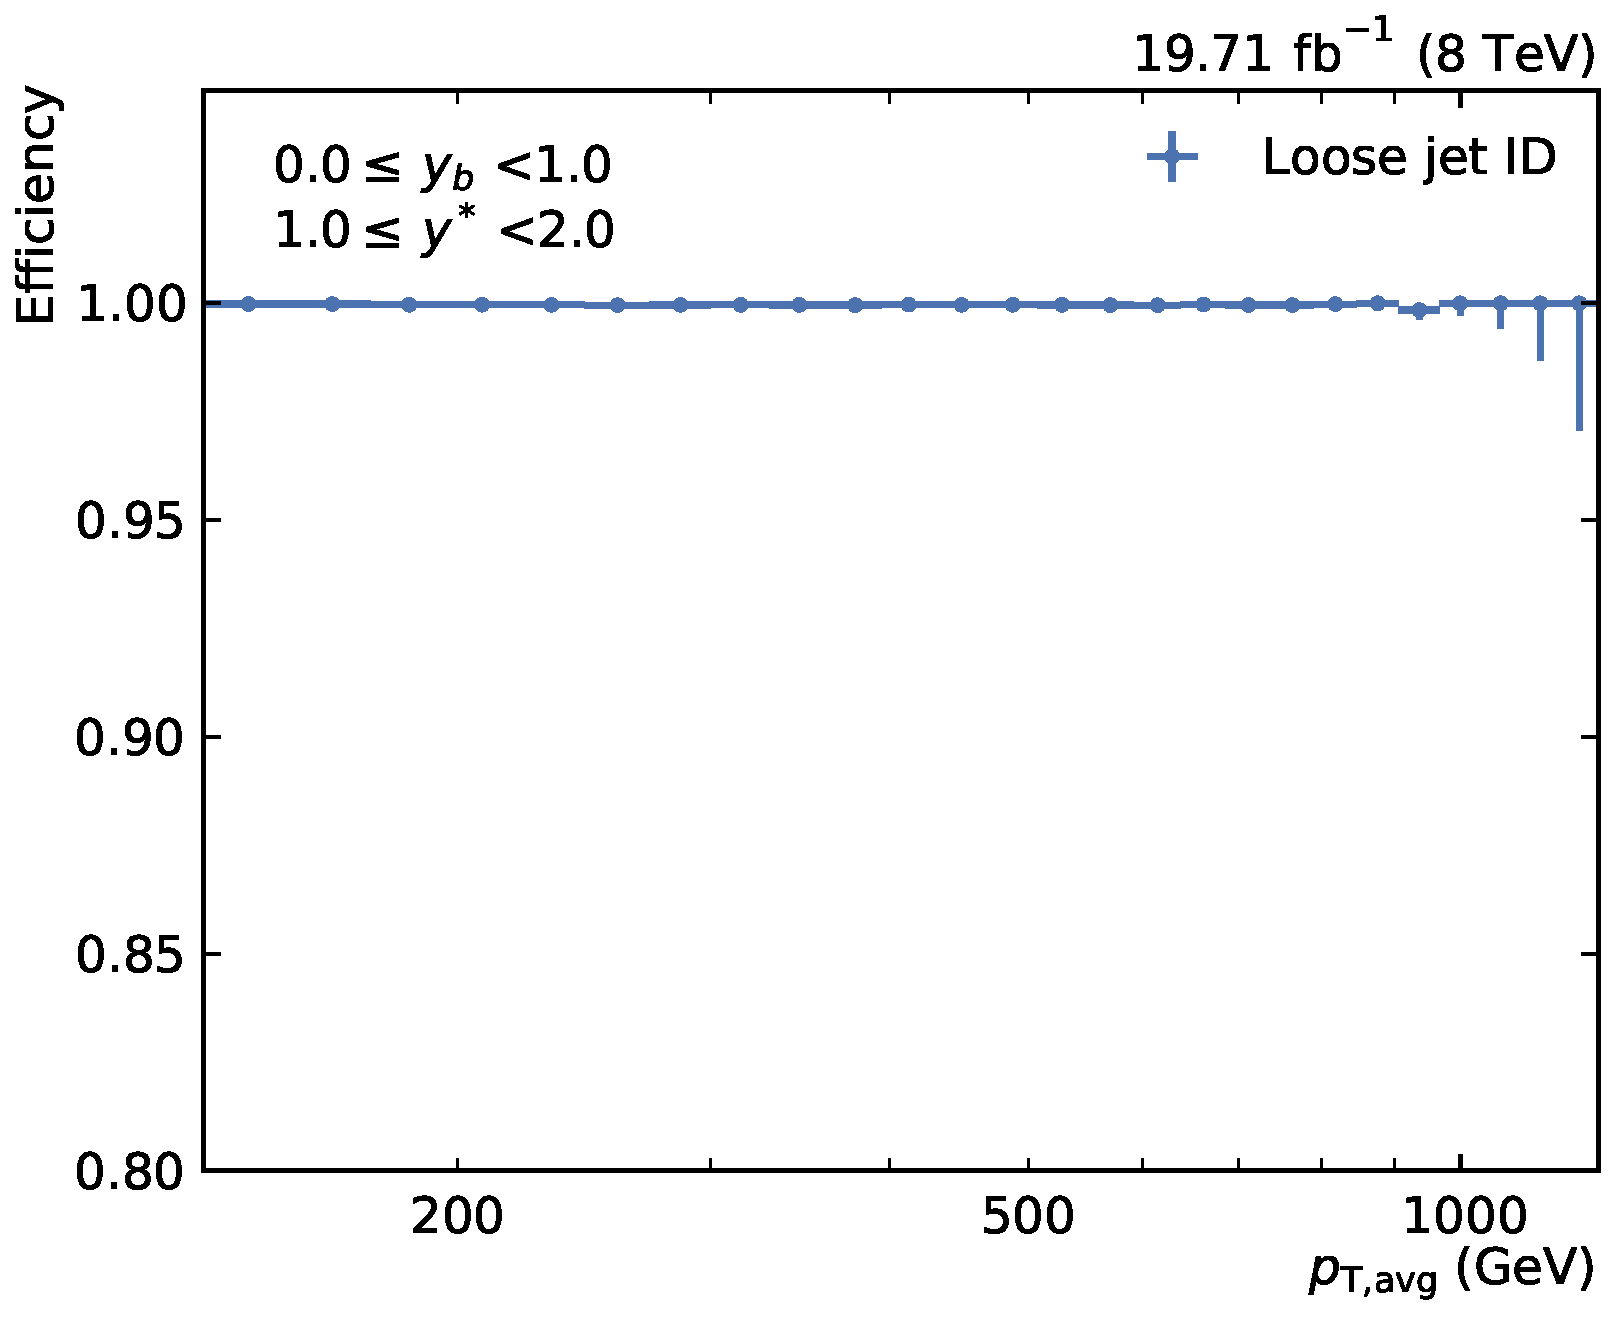
\includegraphics[width=0.45\textwidth]{figures/measurement/jetideff_yb0ys1.pdf}
    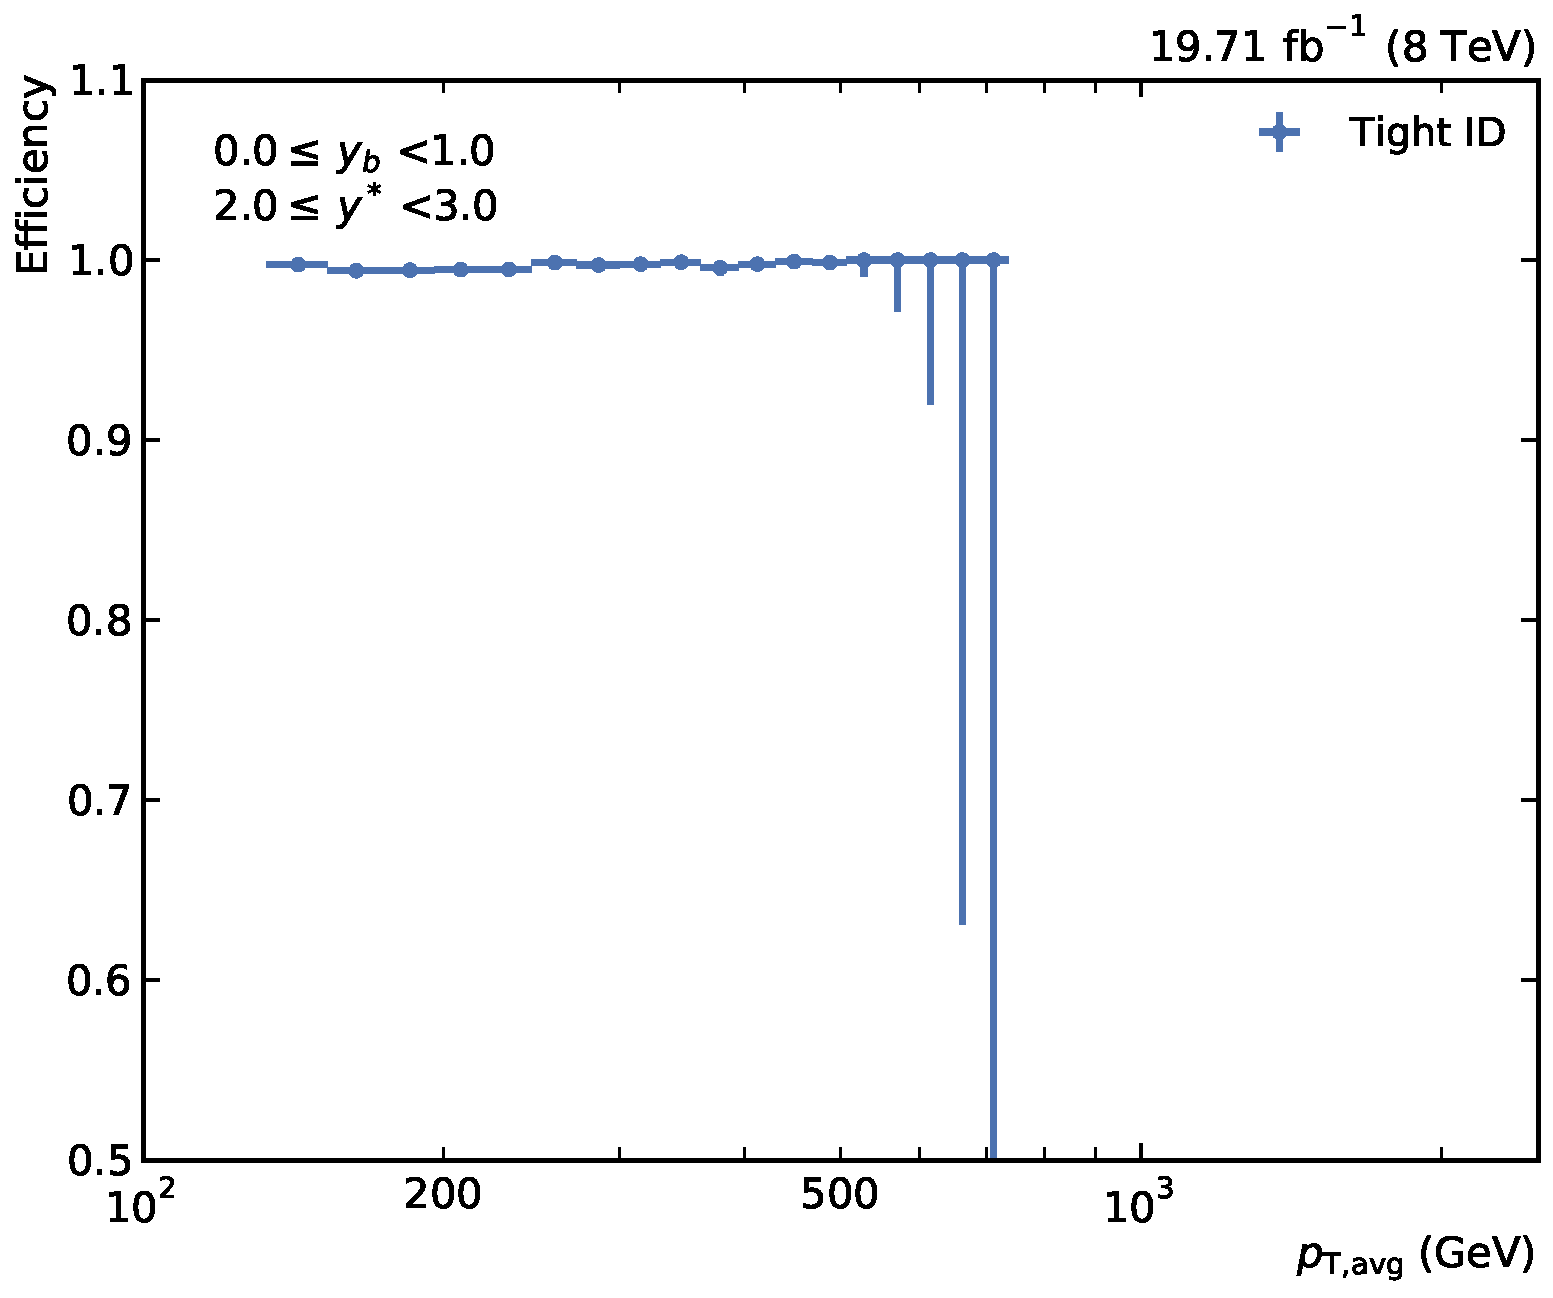
\includegraphics[width=0.45\textwidth]{figures/measurement/jetideff_yb0ys2.pdf}\hfill
    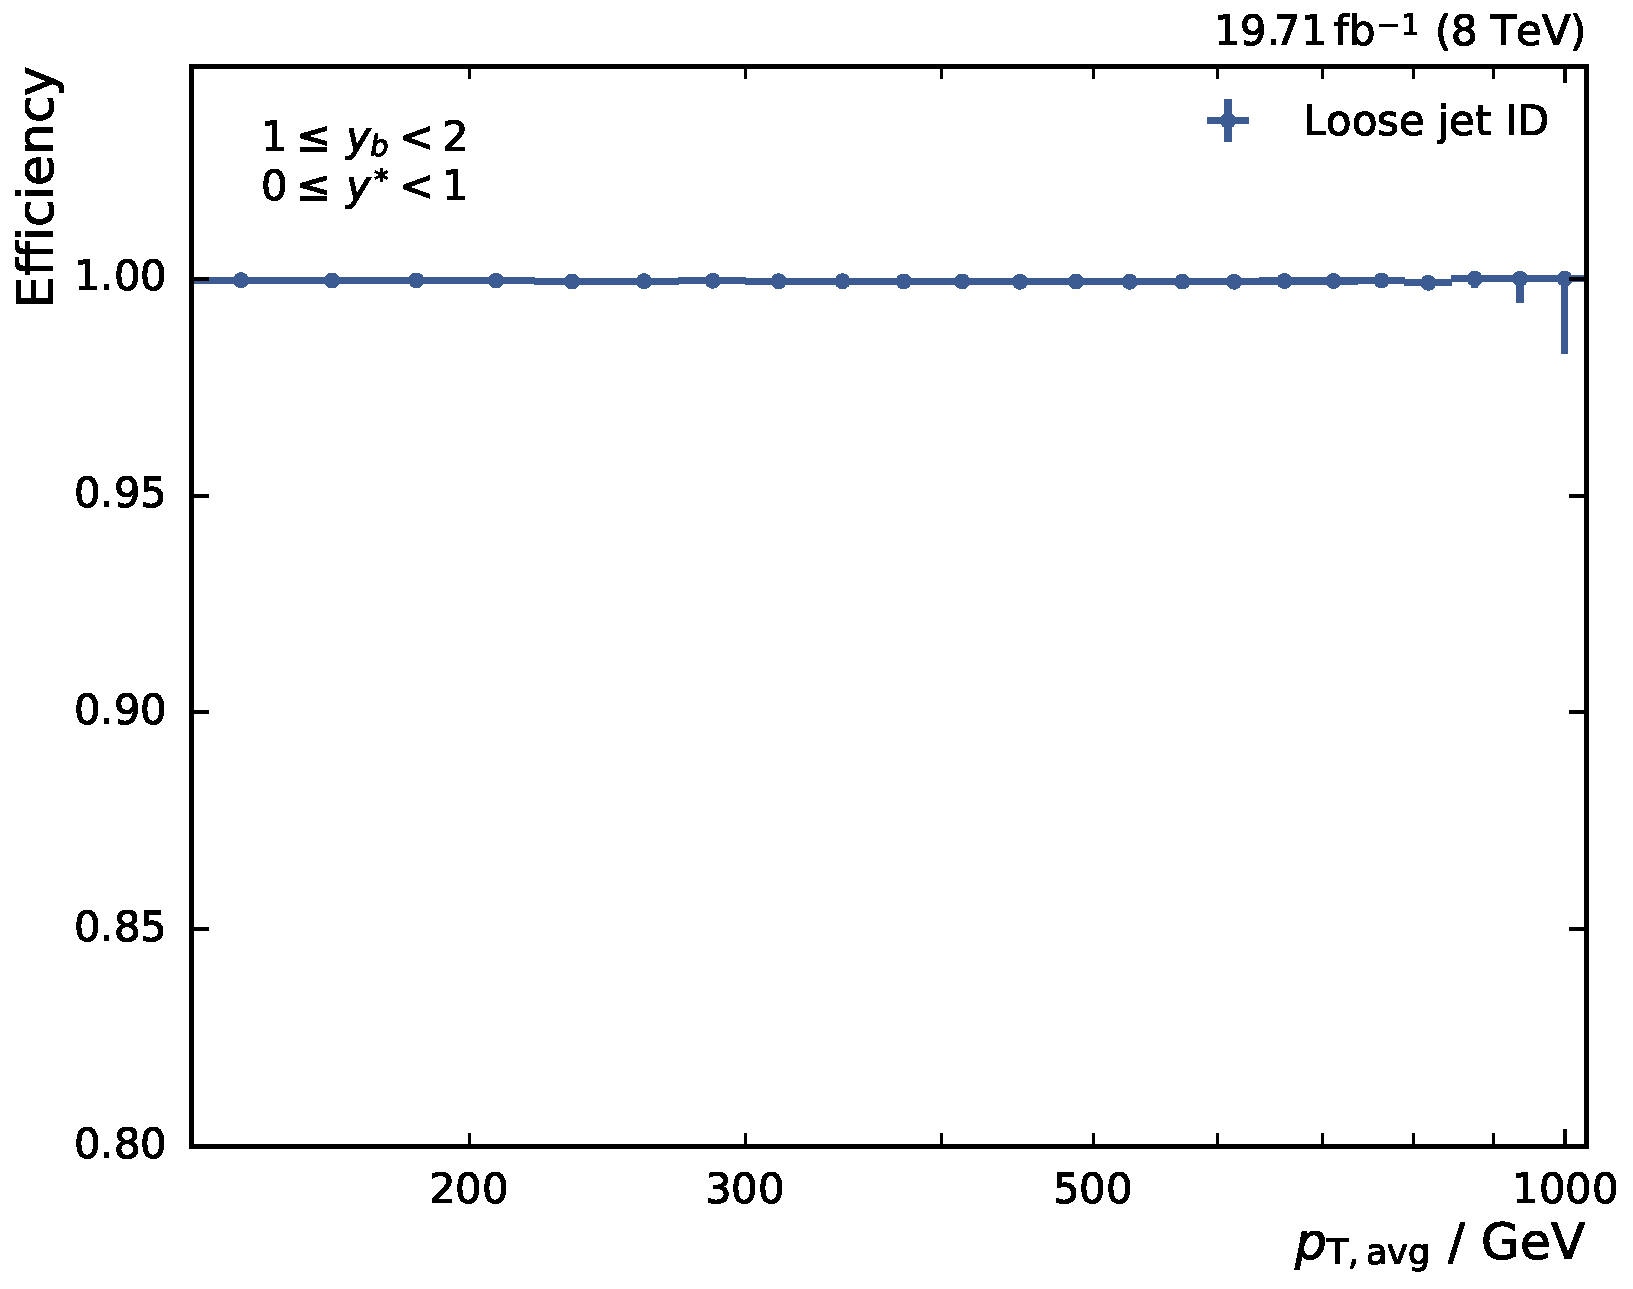
\includegraphics[width=0.45\textwidth]{figures/measurement/jetideff_yb1ys0.pdf}
    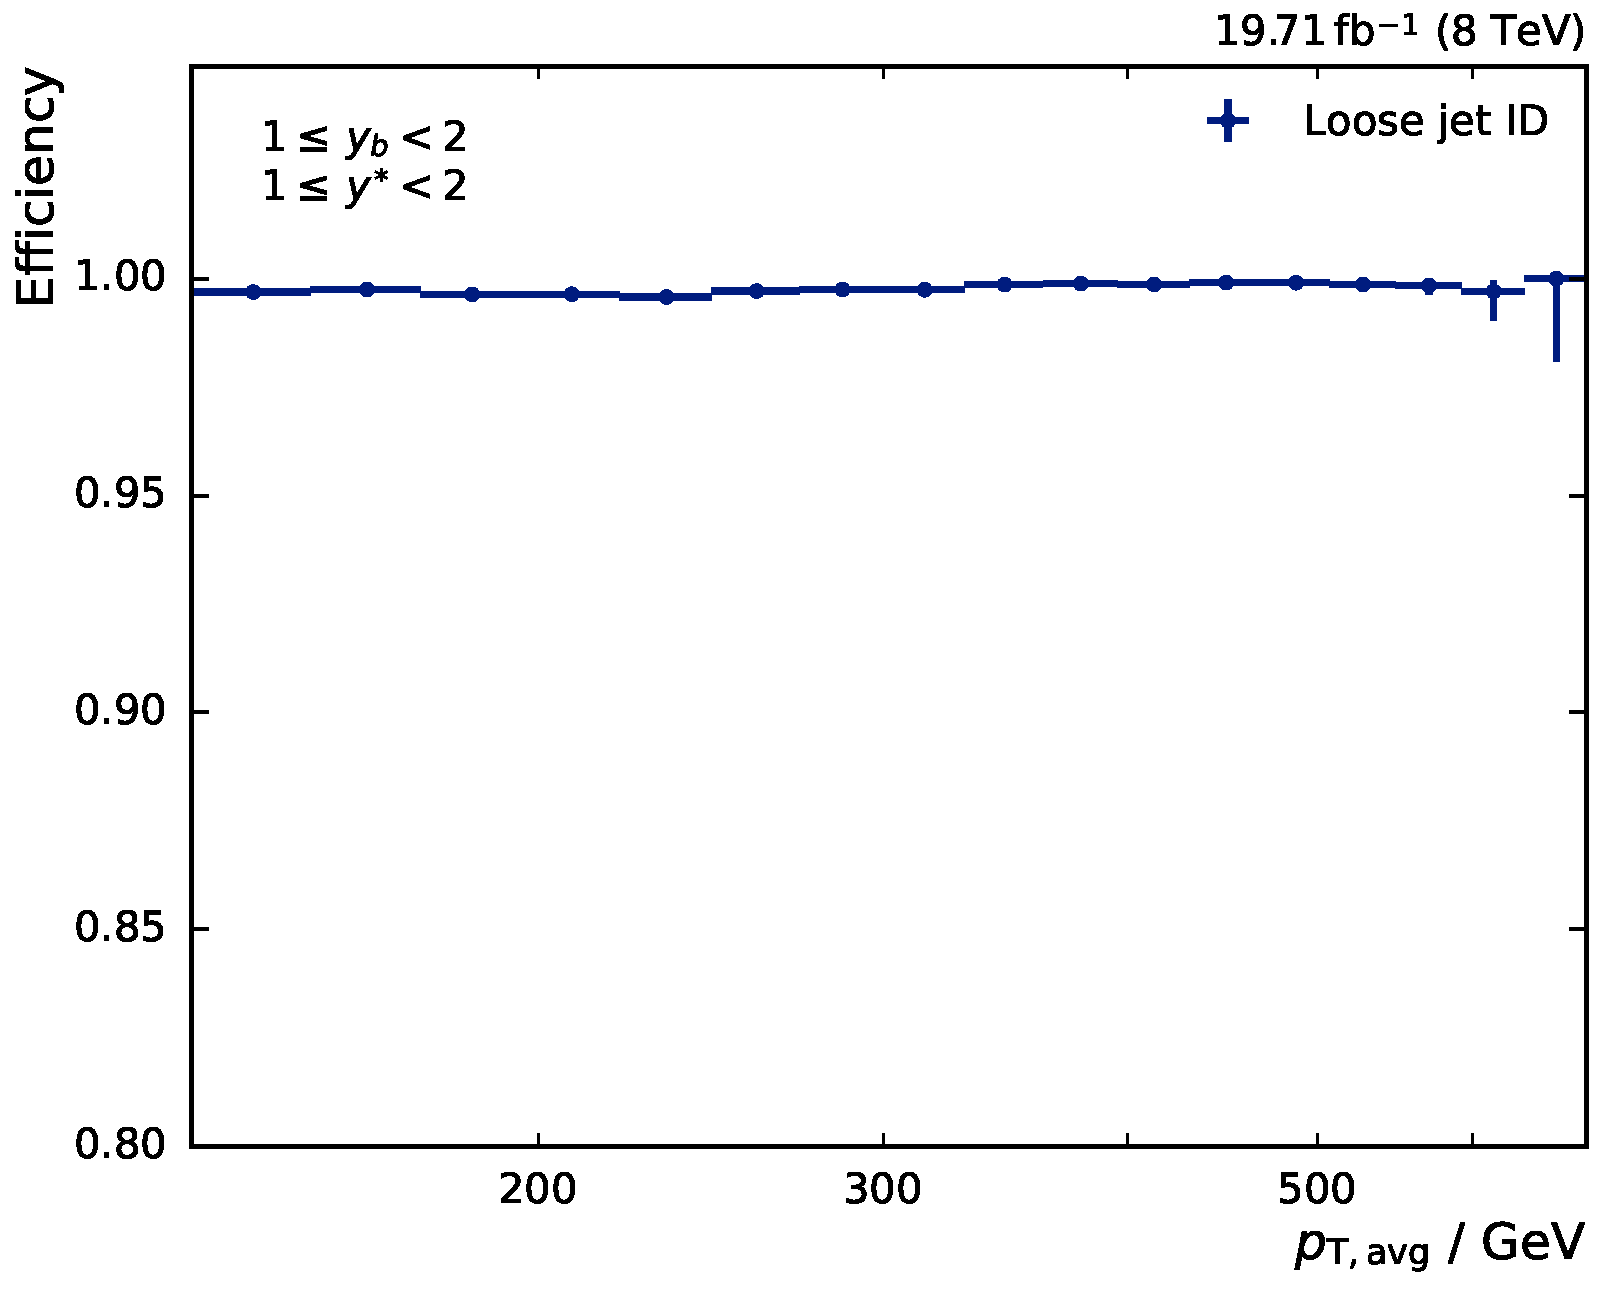
\includegraphics[width=0.45\textwidth]{figures/measurement/jetideff_yb1ys1.pdf}\hfill
    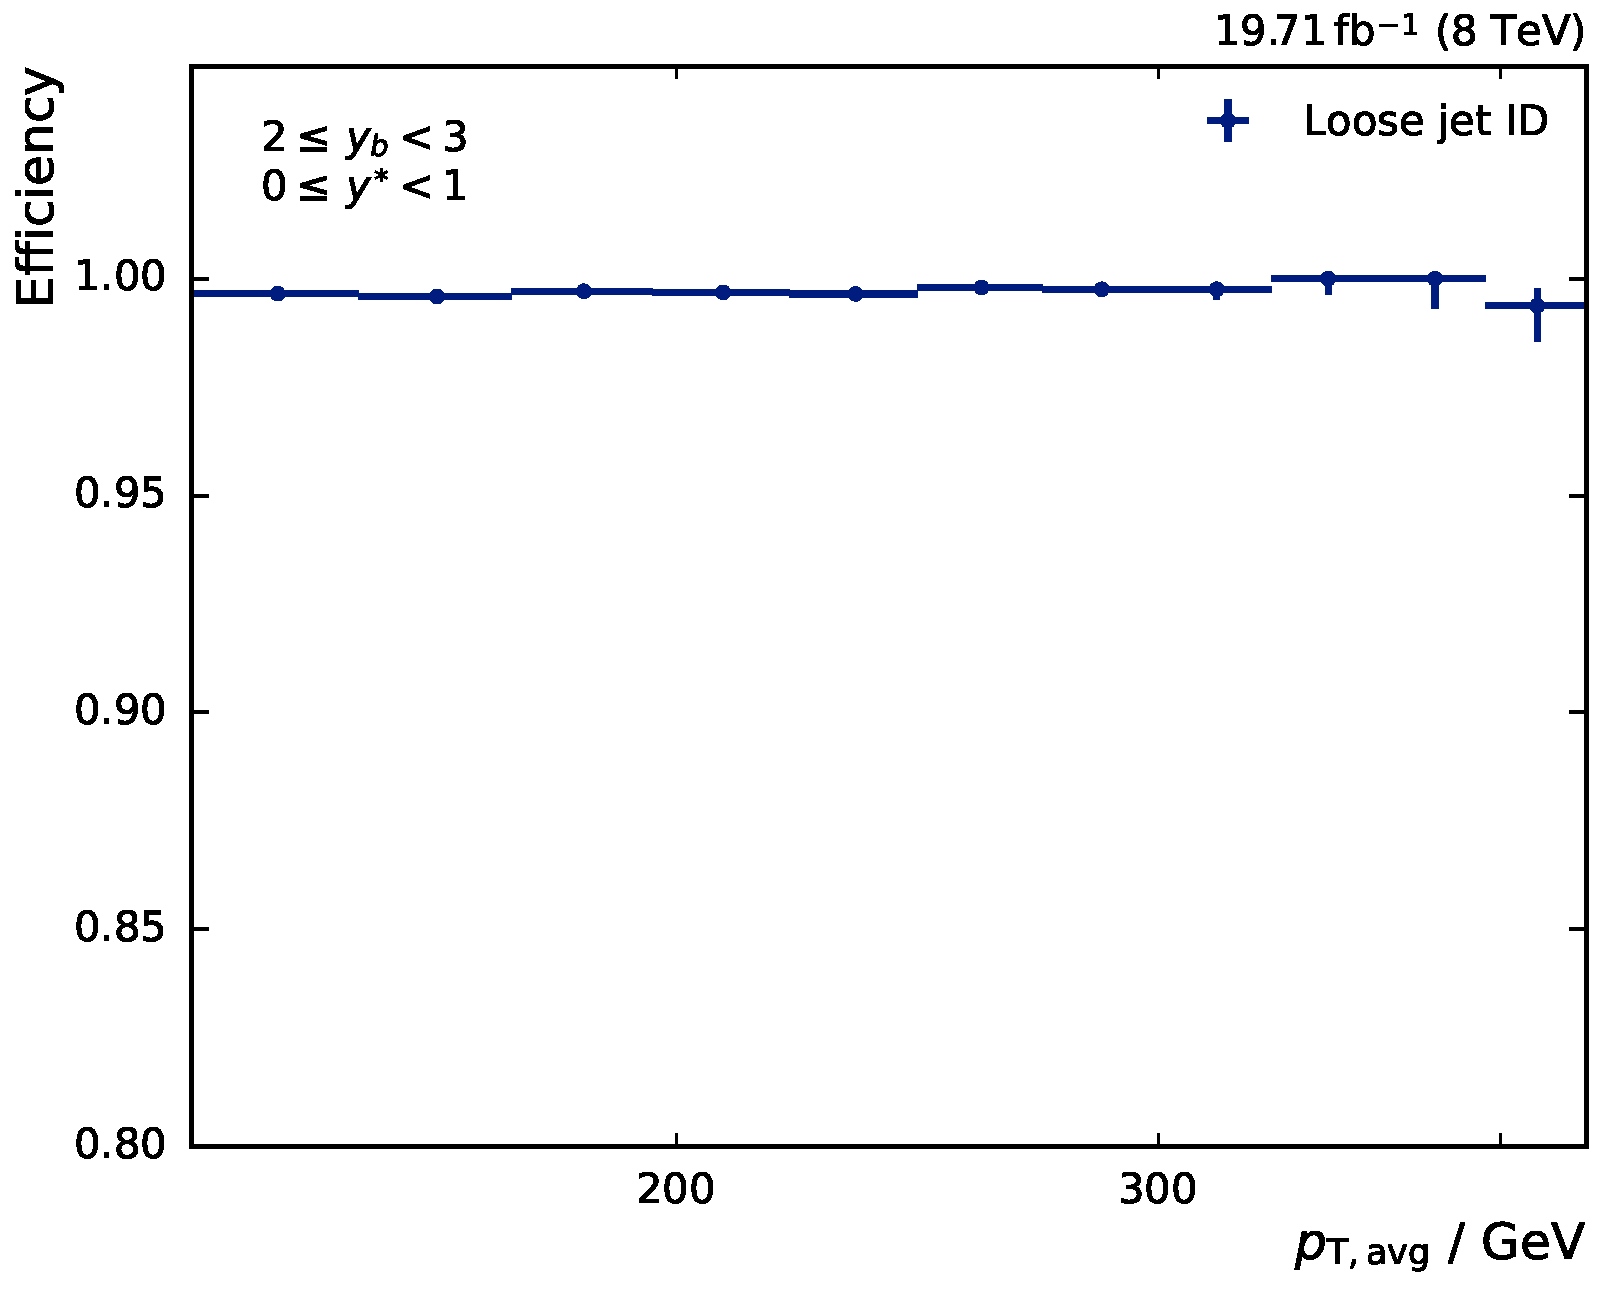
\includegraphics[width=0.45\textwidth]{figures/measurement/jetideff_yb2ys0.pdf}
    \caption{Jet id efficiency studied using a tag-and-probe approach on clear dijet event signatures. The efficiency
    is shown as a function of the average dijet \pt for all bins in \ystar \yboost. The efficiency is in all cases larger
    than 99\%..}
    \label{fig:jetid_eff}
\end{figure}



\cleardoublepage
%\addcontentsline{toc}{chapter}{List of Figures}
\listoffigures

\cleardoublepage
%\addcontentsline{toc}{chapter}{List of Tables}
\listoftables
%\end{comment}

\cleardoublepage
%\addcontentsline{toc}{chapter}{\acronymname}
\printglossary[type=\acronymtype]

\cleardoublepage
% \phantomsection
%\addcontentsline{toc}{chapter}{Bibliography}
%\bibliographystyle{dinat_eng} 
%\bibliographystyle{alphadin}
%\bibliography{includes/papers,includes/images}
\printbibliography

\cleardoublepage

\thispagestyle{empty}
\cleardoublepage
\thispagestyle{empty}
% \chapter*{}
\null\vspace{10cm}
\noindent
{\sffamily \textbf{Erklärung der selbständigen Anfertigung der
Dissertationsschrift}}\\[1cm]

\noindent
Hiermit erkläre ich, dass ich die Dissertationsschrift mit dem Titel
%
\begin{center}
 \guillemotright
 \textit{Measurement of Triple-Differential Dijet Cross Sections\\
            with the CMS Detector at 8 TeV and PDF Constraints}\guillemotleft\\[1.5ex]

\end{center}
%
selbständig und unter ausschließlicher Verwendung der angegebenen Hilfsmittel\\
angefertigt habe.
\vspace{12ex}

\noindent
\hrulefill\hspace{9cm}

\noindent
Georg Sieber\\
\noindent
Karlsruhe, den 04. Mai 2016
% Karlsruhe, den 18. April 2016



